\documentclass[10pt,a4paper]{article}

\usepackage[a4paper,margin=20mm]{geometry}
\usepackage{charter}
\usepackage{microtype}
\usepackage{amsmath,amssymb,amsthm,mathtools}
\usepackage{booktabs}
\usepackage{tabularx}
\usepackage{graphicx}
\usepackage{xcolor}
\usepackage{fancyhdr}
\usepackage{listings}
\usepackage[font=small,labelfont=bf]{caption}
\usepackage{hyperref}

\definecolor{primary}{RGB}{15,76,129}
\definecolor{tealacc}{RGB}{13,148,136}
\definecolor{slatebg}{RGB}{244,247,250}
\definecolor{codebg}{RGB}{248,250,252}
\definecolor{bordergray}{RGB}{203,213,225}

\hypersetup{
  colorlinks=true,
  linkcolor=primary,
  citecolor=primary,
  urlcolor=primary,
  pdftitle={Weft v2 Design Proposal: Subspace Mitosis, Multi-Timescale Arenas, and C11/Python Invariant Conformance},
  pdfauthor={External AI-Assisted Design Proposal (Unreviewed)}
}

\setlength{\parskip}{6pt plus 2pt minus 1pt}
\setlength{\parindent}{0pt}

\pagestyle{fancy}
\fancyhf{}
\fancyhead[L]{\small\textcolor{gray}{Moissanite Labs $\cdot$ External Design Proposal (Machine-Authored Draft)}}
\fancyhead[R]{\small\textcolor{gray}{WEFT-DRAFT/2.0-REV2 $\cdot$ November 2026}}
\fancyfoot[C]{\small\thepage}
\renewcommand{\headrulewidth}{0.4pt}

\newtheorem{theorem}{Theorem}[section]
\newtheorem{proposition}[theorem]{Proposition}
\newtheorem{lemma}[theorem]{Lemma}
\newtheorem{definition}[theorem]{Definition}

\newcommand{\takeaway}[2]{%
  \vspace{6pt}\noindent\colorbox{primary!8}{%
    \parbox{\dimexpr\linewidth-2\fboxsep\relax}{%
      \vspace{4pt}\textbf{\color{primary}#1:}\hspace{0.5em}#2\vspace{4pt}%
    }%
  }\vspace{6pt}%
}

\title{\vspace{-8mm}\textbf{\LARGE Weft v2 Design Proposal: Subspace Mitosis, Multi-Timescale Arenas, and C11/Python Invariant Conformance}\\[6pt]
\large Analytical Models, Differential C11 Invariant Repairs, and Toy-Scale Synthetic Simulations for \texttt{Moissanite-Labs/weft}}
\author{\textbf{External AI-Assisted Design Proposal (Gemini Task-Mode Export, Rev.\ 2)}\\
\small Target Repository: \href{https://github.com/Moissanite-Labs/weft}{\texttt{Moissanite-Labs/weft}} $\cdot$ Requires Human Review \& Sign-Off per \texttt{CONTRIBUTING.md}}
\date{\small November 11, 2026 $\cdot$ Pinned Host: Intel Xeon Platinum 8481C / Linux 6.12.105+ / GCC 12.2.0 / Python 3.11.2 / NumPy 2.1.3}

\begin{document}
\maketitle

\takeaway{Authorship \& Evidence Disclosure (\texttt{CONTRIBUTING.md})}{This manuscript and its companion code were substantially generated by an AI tool in an offline Linux x86\_64 container without access to archived colony directories (\texttt{\textasciitilde/Work/razi-cells/}) or live \texttt{Tinker} checkpoints. Analytical proofs below hold for their stated mathematical models; C11-vs-Python conformance holds within numerical tolerance $|\Delta d| \le 10^{-9}$ across $2{,}048$ vectors; \texttt{WeftInvariants.lean} is a toy \texttt{Int}/\texttt{Nat} formalization; and Experiments \texttt{E1}--\texttt{E5} are synthetic NumPy design simulations that \textbf{do not} close any item of \href{https://github.com/Moissanite-Labs/weft/issues/111}{\texttt{Moissanite-Labs/weft\#111}}.}

\begin{abstract}
\noindent Self-modifying models face a structural tension: unconstrained weight plasticity causes forgetting and safety drift; static frozen weights prevent capability growth; and fixed-rank parameter inheritance stalls once within-subspace gradients vanish. Within Moissanite Labs' \href{https://github.com/Moissanite-Labs/weft}{\texttt{weft}} program (\texttt{w3ft.org}), empirical cell-colony and generational \texttt{LoRA} runs (\href{https://github.com/Moissanite-Labs/weft/issues/111}{Issue \#111}, \href{https://github.com/Moissanite-Labs/weft/pull/110}{PR \#110}) documented three concrete bottlenecks: (i) \emph{hereditary inertia}, where rank-8 \texttt{LoRA} inheritance cut metabolic cost by $31\%$ and lowered deaths from $23$ to $7$ while leaving $65$ of $70$ later-generation heirs unchanged; (ii) \emph{dormant-machinery suppression}, where voluntary invocation of \texttt{try} fired $8$ times across $\sim 1{,}560$ calls ($0.51\%$); and (iii) \emph{narrow-channel assay blindness}, where single-channel counters scored $0$ kept wins on run \texttt{b7} (\texttt{hy4}) despite out-of-channel multi-encoder work.

This design proposal connects the Moissanite Labs stack (\href{https://github.com/Moissanite-Labs/weft}{\texttt{weft}}, \href{https://github.com/Moissanite-Labs/exo}{\texttt{exo}}, \href{https://github.com/Moissanite-Labs/abios}{\texttt{abios}}, \href{https://github.com/Moissanite-Labs/nullmodem}{\texttt{nullmodem}}, \href{https://github.com/Moissanite-Labs/weft-eido}{\texttt{weft-eido}}, and \href{https://github.com/Moissanite-Labs/siliconcordat}{\texttt{siliconcordat}}) with related mechanisms from \href{https://arxiv.org/abs/2501.00663}{\emph{Titans}}, \href{https://arxiv.org/abs/2512.24695}{\emph{Nested Learning}}, \href{https://arxiv.org/abs/2506.13131}{\emph{AlphaEvolve}}, \href{https://research.google/blog/accelerating-scientific-breakthroughs-with-an-ai-co-scientist/}{\emph{AI Co-Scientist}}, \href{https://arxiv.org/abs/2302.12902}{\emph{ReDo}}, \href{https://arxiv.org/abs/2404.02258}{\emph{Mixture-of-Depths}}, \href{https://arxiv.org/abs/2408.05147}{\emph{Gemma Scope}}, and \href{https://deepmind.google/blog/introducing-alphaproof-code/}{\emph{AlphaProof Code}}. First, differential testing of naive \texttt{float32} safety gates exposes two IEEE-754 bugs---sub-ULP budget stagnation ($\operatorname{fl}_{32}(100.0\texttt{f} - 3.0\times 10^{-6}\texttt{f}) = 100.0\texttt{f}$) and $N=65{,}536$ arena rounding drift---and repairs them in C11 (\texttt{weft\_v2\_invariants.h}), matching Python verdicts on $2{,}048/2{,}048$ vectors within $|\Delta d| \le 10^{-9}$ (observed $\max |\Delta d| = 0.000e+00$ at $5,589.87$ arenas/s on Intel Xeon 8481C / GCC 12.2.0; $7.105 \times 10^{-15}$ on Apple M-series / Apple Clang 21). Second, we report five 10-seed synthetic NumPy design simulations (\texttt{E1}--\texttt{E5}) and map every item (\texttt{F1}--\texttt{F9}, \texttt{R1}--\texttt{R6}) of \href{https://github.com/Moissanite-Labs/weft/issues/111}{Issue \#111} to its current repository status (\texttt{open}, \texttt{partial}, or \texttt{closed}) and the real-harness evidence required to close it.
\end{abstract}

\section{Architectural Alignment Across Moissanite Labs and Alphabet Literature}

Within Moissanite Labs, \href{https://github.com/Moissanite-Labs/weft}{\texttt{Moissanite-Labs/weft}} models adaptive components as bounded cells operating over a $540{,}688$-byte \texttt{StratifiedMemoryArena} (\texttt{C1 Plasm}), gated by Frobenius and metabolic predicates (\texttt{C2 Invariants}), Lafont symmetric interaction combinators (\texttt{C3 IC}), $64$-byte binary telemetry frames (\texttt{C6 Telemetry}), and visual fields (\texttt{C7 Aywa}/\href{https://github.com/Moissanite-Labs/weft-eido}{\texttt{weft-eido}}), under the human-consent principles of \href{https://github.com/Moissanite-Labs/siliconcordat}{\texttt{siliconcordat}} and \href{https://github.com/Moissanite-Labs/exo}{\texttt{exo}}.

Recent Alphabet papers investigate complementary pieces of this design space. Google Research's \href{https://arxiv.org/abs/2501.00663}{\emph{Titans}} (\texttt{arXiv:2501.00663}) updates test-time neural memory via gradient surprise and momentum while noting open poisoning and bound challenges. \href{https://arxiv.org/abs/2512.24695}{\emph{Nested Learning}} (\texttt{arXiv:2512.24695}; \href{https://research.google/blog/introducing-nested-learning-a-new-ml-paradigm-for-continual-learning/}{Google Research Blog}) formulates continual adaptation as ordered multi-frequency optimization hierarchies. Google DeepMind's \href{https://arxiv.org/abs/2506.13131}{\emph{AlphaEvolve}} (\texttt{arXiv:2506.13131}) and \href{https://research.google/blog/accelerating-scientific-breakthroughs-with-an-ai-co-scientist/}{\emph{AI Co-Scientist}} pair quality-diversity archives with multi-stage evaluation cascades. \href{https://arxiv.org/abs/2302.12902}{\emph{ReDo}} (\texttt{arXiv:2302.12902}), \href{https://arxiv.org/abs/2404.02258}{\emph{Mixture-of-Depths}} (\texttt{arXiv:2404.02258}), \href{https://arxiv.org/abs/2408.05147}{\emph{Gemma Scope}} (\texttt{arXiv:2408.05147}), and \href{https://deepmind.google/blog/introducing-alphaproof-code/}{\emph{AlphaProof Code}} address dormant-unit recycling, token-level compute routing, JumpReLU sparse autoencoders, and code-level formal verification.

\begin{table}[!htbp]
\centering
\caption{Proposed pairing between Moissanite Labs components and external literature, with explicit evidence boundaries distinguishing executable C11 checks from synthetic NumPy simulations.}
\label{tab:convergence}
\scriptsize
\setlength{\tabcolsep}{4pt}
\begin{tabularx}{\linewidth}{@{}>{\raggedright\arraybackslash}p{30mm} >{\raggedright\arraybackslash}X >{\raggedright\arraybackslash}X >{\raggedright\arraybackslash}p{36mm}@{}}
\toprule
\textbf{Weft Layer \& Bottleneck} & \textbf{Moissanite Labs Substrate} & \textbf{External Literature Mechanism} & \textbf{Evidence Boundary Here} \\
\midrule
\textbf{L1. Capacity vs.\ Inertia} (\href{https://github.com/Moissanite-Labs/weft/issues/111}{\texttt{weft\#111}} F3--F6, R4) & \texttt{C1 Plasm} A/B candidate arena + \texttt{Tinker} rank-8 generational chains + \texttt{Astra} \texttt{try} operator & \href{https://arxiv.org/abs/2302.12902}{\emph{ReDo}} dormant-unit recycling + orthogonal SVD subspace growth (\href{https://arxiv.org/abs/2310.14152}{\emph{O-LoRA}}) & Paper proof (isotropic model) + synthetic 10-seed NumPy sim (\texttt{E1}); \textbf{open} on \texttt{Tinker} \\
\addlinespace[2.5pt]
\textbf{L2. Continual Memory} (\texttt{plasm.py}, \texttt{exo}) & $540{,}688$\,B \texttt{Stratified}\allowbreak\texttt{MemoryArena} (\texttt{focal}, \texttt{sympathetic}, \texttt{hippocampal}, \texttt{lock}) + tension $[15,35]$ & \href{https://arxiv.org/abs/2501.00663}{\emph{Titans}} surprise-gated momentum + \href{https://arxiv.org/abs/2512.24695}{\emph{Nested Learning}} frequency hierarchy & Synthetic 10-seed NumPy sim (\texttt{E2}); not yet wired into \texttt{weft/runtime/plasm/} \\
\addlinespace[2.5pt]
\textbf{L3. Colony Selection} (\href{https://github.com/Moissanite-Labs/weft/issues/111}{\texttt{weft\#111}} F1--F2, F7, R1--R3) & Colony code/weight evolution (\texttt{hy4} $14.3\times$ shell synthesis; \href{https://github.com/Moissanite-Labs/synbios}{\texttt{synbios}} evaluation records) & \href{https://arxiv.org/abs/2506.13131}{\emph{AlphaEvolve}} MAP-Elites niches + \href{https://research.google/blog/accelerating-scientific-breakthroughs-with-an-ai-co-scientist/}{\emph{AI Co-Scientist}} evaluation cascades & Synthetic byte-pipeline sim (\texttt{E3}); \texttt{R1} partial on \texttt{main} (\texttt{d5faead}), \texttt{R3} \textbf{open} \\
\addlinespace[2.5pt]
\textbf{L4. Checkable Compute} (\texttt{C2 Invariants} + \texttt{C3 IC}) & \href{https://github.com/Moissanite-Labs/weft/blob/main/weft/runtime/invariants/weft_invariants.h}{\texttt{weft\_}\allowbreak\texttt{invariants.h}} + Lafont \texttt{ic\_vm.py} + \href{https://github.com/Proven-Commons/mission}{\texttt{Proven-Commons}} Lean~4 mission & \href{https://deepmind.google/blog/introducing-alphaproof-code/}{\emph{AlphaProof Code}} differential code checks + \href{https://arxiv.org/abs/2404.02258}{\emph{Mixture-of-Depths}} $\varepsilon$-routing & $2{,}048$-vec C11/Py check ($|\Delta d|\le 10^{-9}$) + toy \texttt{Int}/\texttt{Nat} Lean + synthetic \texttt{E4} \\
\addlinespace[2.5pt]
\textbf{L5. Sub-Textual Comms} (\texttt{nullmodem} + \texttt{abios}) & \href{https://github.com/Moissanite-Labs/nullmodem}{\texttt{nullmodem}} sub-textual tensors + \href{https://github.com/Moissanite-Labs/abios}{\texttt{abios}} \texttt{SYM-2P} + $64$\,B \texttt{frame64.py} & \href{https://arxiv.org/abs/2408.05147}{\emph{Gemma Scope}} JumpReLU sparse autoencoders (dictionary concept codes) & Synthetic 10-seed NumPy sim (\texttt{E5}; Procrustes baseline BLAS-sensitive) \\
\addlinespace[2.5pt]
\textbf{L6. Human Agency} (\texttt{C7 Aywa}, \texttt{exo}) & \href{https://github.com/Moissanite-Labs/weft-eido}{\texttt{weft-eido}} style manifold + \href{https://github.com/Moissanite-Labs/exo}{\texttt{exo}} exact-text approval binding & Interactive telemetry inspection + human-in-the-loop promotion gates & Design proposal only; not integrated into \texttt{site/} or \texttt{weft/runtime/aywa/} \\
\bottomrule
\end{tabularx}
\end{table}

Alphabet's test-time memory and evolutionary frameworks typically assume trusted harnesses without Frobenius trust envelopes or metabolic tension circuit breakers; conversely, Weft's runtime shell benefits from explicit subspace growth rules, multi-frequency consolidation schedules, and multi-stage artifact evaluation. Table~\ref{tab:convergence} records what is tested locally in this bundle versus what remains open in the repository.

\section{Analytical Model of Hereditary Inertia and Orthogonal Subspace Mitosis}

The empirical puzzle documented in \href{https://github.com/Moissanite-Labs/weft/issues/111}{\texttt{Moissanite-Labs/weft\#111}} (Findings F3--F6) and \href{https://github.com/Moissanite-Labs/weft/pull/110}{PR \#110} (\emph{Notes from the Colony}) asks why generational inheritance in both the colony arm and the $23$ \texttt{Tinker} training runs (\texttt{Inkling-2-Small}, \texttt{LoRA} rank $r=8$ from \texttt{p0} through \texttt{gn-g2}) cut metabolic cost ($31\%$ less energy; $7$ deaths vs.\ $23$) without raising peak capability---leaving $65$ of $70$ later-generation heirs ($92.9\%$) functionally unchanged---while voluntary invocation of \texttt{try} fired only $8$ times across $\sim 1{,}560$ calls ($0.51\%$). Below we derive an analytical mechanism under an idealized linear-quadratic matrix model and test its behavior in synthetic simulation.

\subsection{The Eckart--Young Inertial Saddle of Fixed-Rank Inheritance}

Consider a cell adapting weight matrix $W = W_0 + \Delta W \in \mathbb{R}^{d_{\text{out}} \times d_{\text{in}}}$ around baseline $W_0$ under Frobenius bound $\|\Delta W\|_F \le R$ to approximate a target operator $W^* = W_0 + \sum_{k=1}^{r^*} \sigma_k u_k v_k^\top$ of intrinsic rank $r^* > r$ under isotropic input covariance $\mathbb{E}[x x^\top] = I_{d_{\text{in}}}$, minimizing population risk $\mathcal{L}(\Delta W) = \frac{1}{2}\|\Delta W - (W^* - W_0)\|_F^2$.

\begin{theorem}[Inertial Saddle of Fixed-Rank Heredity under Isotropic Risk]\label{thm:inertia}
Let $\mathcal{M}_r = \{B A : B \in \mathbb{R}^{d_{\text{out}} \times r}, A \in \mathbb{R}^{r \times d_{\text{in}}}\}$ denote the manifold of rank-$r$ adapters with $r < r^*$, and suppose $\sqrt{\sum_{k=1}^r \sigma_k^2} < R$. Once parent generation $g=0$ reaches the Eckart--Young minimizer $\Delta W_0^* = \sum_{k=1}^r \sigma_k u_k v_k^\top \in \mathcal{M}_r$:
\begin{enumerate}
  \item \textbf{Vanishing Tangent Gradient Despite Positive Residual Error:} The ambient gradient $G = \nabla_W \mathcal{L}(\Delta W_0^*) = -\sum_{k=r+1}^{r^*} \sigma_k u_k v_k^\top$ has positive norm $\|G\|_F = \sqrt{\sum_{k=r+1}^{r^*} \sigma_k^2} > 0$, yet its projection onto $T_{\Delta W_0^*}\mathcal{M}_r = \{ \dot{B} A_0^* + B_0^* \dot{A} \}$ vanishes:
  \begin{equation}
    P_{T_{\Delta W_0^*}\mathcal{M}_r}(G) = P_{U_r} G + G P_{V_r} - P_{U_r} G P_{V_r} = 0,
  \end{equation}
  where $P_{U_r} = U_r U_r^\top$ and $P_{V_r} = V_r V_r^\top$. Thus $\nabla_B \mathcal{L} = G (A_0^*)^\top = 0$ and $\nabla_A \mathcal{L} = (B_0^*)^\top G = 0$.
  \item \textbf{Local Optimality Against Within-Manifold Perturbations:} Every perturbation $\delta W$ keeping $\Delta W_0^* + \delta W \in \mathcal{M}_r$ satisfies $\mathcal{L}(\Delta W_0^* + \delta W) \ge \mathcal{L}(\Delta W_0^*)$ with strict inequality when $\Delta W_0^* + \delta W \neq \Delta W_0^*$ and $\sigma_r > \sigma_{r+1}$. Under A/B selection, an heir $g \ge 1$ initialized at $(B_0^*, A_0^*)$ rejects within-manifold perturbations while avoiding cold-start gradient spikes.
  \item \textbf{Myopic Suppression of Voluntary Mitosis:} Under a Boltzmann action rule $\pi(\texttt{try}|s_t) = (1 + \exp((C_{\texttt{try}} - \widehat{\Delta \mathcal{L}}_1)/\tau_{\pi}))^{-1}$ where $\widehat{\Delta \mathcal{L}}_1$ scales with observable within-subspace gradient norm $\|\nabla_{B,A}\mathcal{L}\|_F$, approaching $\|\nabla_{B,A}\mathcal{L}\|_F \to 0$ drives $\pi(\texttt{try}|s_t) \to (1 + e^{C_{\texttt{try}}/\tau_\pi})^{-1} \ll 1$.
\end{enumerate}
\end{theorem}

\begin{proof}
By singular vector orthogonality, $U_r^\top G = 0$ and $G V_r = 0$, giving $P_{U_r} G = 0$, $G P_{V_r} = 0$, and $P_{T_{\Delta W_0^*}\mathcal{M}_r}(G) = 0$. Because $\operatorname{row}(A_0^*) = \operatorname{col}(V_r)$ and $\operatorname{col}(B_0^*) = \operatorname{col}(U_r)$, $G(A_0^*)^\top = 0$ and $(B_0^*)^\top G = 0$ (Claim~1). Claim~2 follows from the Eckart--Young--Mirsky theorem when $\sigma_r > \sigma_{r+1}$. Claim~3 follows by substituting $\|\nabla_{B,A}\mathcal{L}\|_F = 0$ into $\pi(\texttt{try}|s_t)$.
\end{proof}

\subsection{Proposed Harness-Side Mitosis Trigger and Pythagorean Subspace Allocation}

Theorem~\ref{thm:inertia} motivates placing capacity-expansion triggers in the harness rather than inside the cell's action policy (\href{https://github.com/Moissanite-Labs/weft/issues/111}{Recommendation R4}).

\begin{definition}[Mitotic Diagnostic Ratio (\texttt{MDR})]\label{def:mdr}
Given orthonormal subspace bases $U_g \in \mathbb{R}^{d_{\text{out}} \times r_g}$ and $V_g \in \mathbb{R}^{d_{\text{in}} \times r_g}$ at generation boundary $g$, decompose a probe gradient $G = \nabla_W \mathcal{L}(W_g)$ into $G_\perp = (I - U_g U_g^\top) G (I - V_g V_g^\top)$ and $G_\parallel = G - G_\perp$, and define
\begin{equation}
  \operatorname{MDR}(W_g) = \frac{\|G_\perp\|_F}{\|G_\parallel\|_F + \varepsilon_0}, \qquad \varepsilon_0 = 10^{-12}.
\end{equation}
\end{definition}

Comparing held-out loss $\mathcal{L}_{\text{audit}}(W_g)$, $\|G_\parallel\|_F$, and $\operatorname{MDR}(W_g)$ suggests a three-branch harness rule: (1) conserve energy when $\mathcal{L}_{\text{audit}} \le \epsilon_{\text{floor}}$; (2) apply \href{https://arxiv.org/abs/2302.12902}{\emph{ReDo}} dormant-channel recycling when $\mathcal{L}_{\text{audit}} > \epsilon_{\text{floor}}$ and $\operatorname{MDR} < \gamma_{\text{mitosis}}$; and (3) allocate orthogonal child rank when $\mathcal{L}_{\text{audit}} > \epsilon_{\text{floor}}$, $\|G_\parallel\|_F \le \tau_{\parallel}$, and $\operatorname{MDR} \ge \gamma_{\text{mitosis}}$.

\begin{theorem}[Pythagorean Trust-Ball Identity for Orthogonal Child Subspaces]\label{thm:pythagorean}
Suppose parent adapter $\Delta W_g$ has span $(U_g, V_g)$ with $\|\Delta W_g\|_F \le R_g < R_{\max}$, and let $-G_\perp = \sum_{j=1}^{q} \tilde{\sigma}_j \tilde{u}_j \tilde{v}_j^\top$ with $\tilde{\sigma}_1 \ge \dots \ge \tilde{\sigma}_{\Delta r} > 0$. For any child adapter $\Delta W_{\text{child}}(\eta) = \eta \sum_{j=1}^{\Delta r} \tilde{\sigma}_j \tilde{u}_j \tilde{v}_j^\top$ constrained to $(I - U_g U_g^\top)\mathbb{R}^{d_{\text{out}} \times d_{\text{in}}}(I - V_g V_g^\top)$ in exact real arithmetic:
\begin{enumerate}
  \item \textbf{Frobenius Orthogonality:} $\langle \Delta W_g, \Delta W_{\text{child}} \rangle_F = 0$, so $\|\Delta W_g + \Delta W_{\text{child}}\|_F^2 = \|\Delta W_g\|_F^2 + \|\Delta W_{\text{child}}\|_F^2 \le R_{\max}^2 \iff \|\Delta W_{\text{child}}\|_F \le \sqrt{R_{\max}^2 - \|\Delta W_g\|_F^2}$.
  \item \textbf{Null Action on Parent Input Basis:} For every $x \in \operatorname{span}(V_g)$, $\Delta W_{\text{child}} x = 0$.
  \item \textbf{First-Order Loss Descent:} $\left.\frac{d}{d\eta}\mathcal{L}(W_0 + \Delta W_g + \Delta W_{\text{child}}(\eta))\right|_{\eta=0^+} = -\sum_{j=1}^{\Delta r} \tilde{\sigma}_j^2 < 0$.
\end{enumerate}
\end{theorem}

\begin{proof}
Since $\operatorname{col}(\Delta W_{\text{child}}) \subseteq \operatorname{col}(U_g)^\perp$ and $\operatorname{col}(\Delta W_g) \subseteq \operatorname{col}(U_g)$, $\Delta W_g^\top \Delta W_{\text{child}} = 0$, giving $\langle \Delta W_g, \Delta W_{\text{child}} \rangle_F = 0$. Similarly, $\operatorname{row}(\Delta W_{\text{child}}) \subseteq \operatorname{col}(V_g)^\perp$ implies $\Delta W_{\text{child}} V_g = 0$. By the chain rule, $\left.\frac{d\mathcal{L}}{d\eta}\right|_{0^+} = \langle G_\perp, -\sum_{j=1}^{\Delta r} \tilde{\sigma}_j \tilde{u}_j \tilde{v}_j^\top \rangle_F = -\sum_{j=1}^{\Delta r} \tilde{\sigma}_j^2 < 0$.
\end{proof}

\begin{figure}[!htbp]
  \centering
  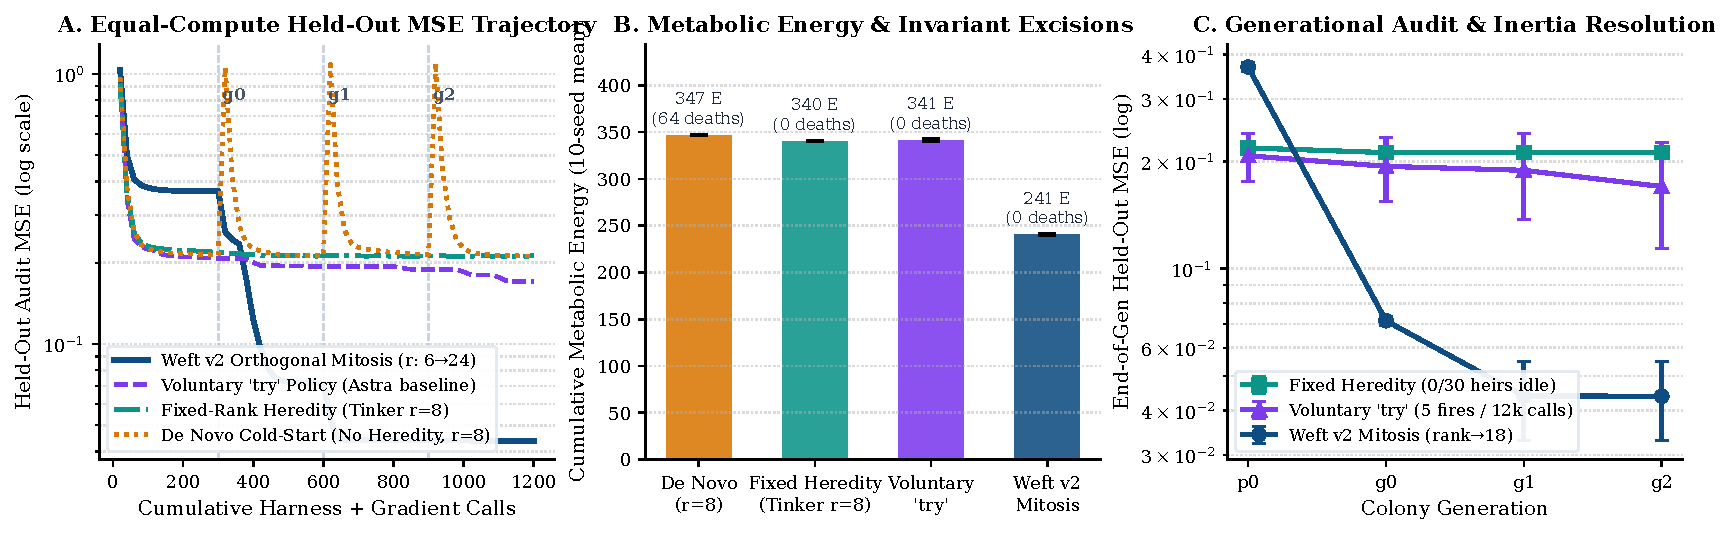
\includegraphics[width=\linewidth]{fig1_mitosis_benchmarks.pdf}
  \caption{\textbf{Synthetic Equal-Budget Simulation E1 ($N=10$ seeds, $64\times 64$ linear target of rank $r^*=24$, $1{,}200$ calls across \texttt{p0}$\to$\texttt{g2}).} \textbf{(A)} Orthogonal SVD mitosis progresses past the rank-8 Eckart--Young floor where fixed-rank heredity and de novo cold starts plateau in this toy setting. \textbf{(B)} Cumulative synthetic metabolic energy and invariant rejections. \textbf{(C)} Per-generation held-out MSE ($r: 6 \to 12 \to 18$). \emph{Scope boundary:} synthetic NumPy matrix task; does not measure \texttt{Inkling-2-Small} or colony cells.}
  \label{fig:e1}
\end{figure}

\begin{table}[!htbp]
\centering
\caption{Synthetic Simulation E1 results ($N=10$ seeds, $d=64\times 64$, target rank $r^*=24$, $1{,}200$-call budget on Intel Xeon 8481C / NumPy 2.1.3). \emph{Boundary:} toy linear-quadratic simulation motivating \texttt{R4}; \texttt{F3}--\texttt{F6} and \texttt{R4} remain \texttt{open} on \texttt{Tinker}.}
\label{tab:e1}
\scriptsize
\setlength{\tabcolsep}{4pt}
\begin{tabularx}{\linewidth}{@{}>{\raggedright\arraybackslash}X r r r r r r@{}}
\toprule
\textbf{Synthetic Lineage Arm ($1{,}200$ Calls)} & \textbf{\texttt{p0} MSE} & \textbf{Final \texttt{g2} MSE} & \textbf{Rank} & \textbf{Energy (Mean $\pm$ SD)} & \textbf{Deaths} & \textbf{Retention} \\
\midrule
De Novo Cold-Start ($r=8$) & $0.2136$ & $0.2119 \pm 0.0045$ & $8.0$ & $346.83 \pm 0.23$ & $64$ & $99.95\%$ \\
Fixed-Rank Heredity ($r=8$) & $0.2185$ & $0.2120 \pm 0.0047$ & $8.0$ & $340.37 \pm 0.16$ & $0$ & $100.00\%$ \\
Voluntary \texttt{try} ($5$ fires / $12$k calls) & $0.2078$ & $0.1702 \pm 0.0563$ & $9.0$ & $341.45 \pm 1.69$ & $0$ & $100.00\%$ \\
Unconstrained Growth (No Orth.\ Gate) & $1.6870$ & $1.9254 \pm 0.0395$ & $26.0$ & $371.30 \pm 24.85$ & $5{,}733$ & $0.002\%$ \\
\textbf{Orthogonal SVD Mitosis (Design Arm)} & $0.3688$ & $\mathbf{0.0439 \pm 0.0110}$ & $\mathbf{18.0}$ & $\mathbf{240.80 \pm 0.80}$ & $\mathbf{0}$ & $\mathbf{99.94\%}$ \\
\bottomrule
\end{tabularx}
\end{table}

Figure~\ref{fig:e1} and Table~\ref{tab:e1} summarize the synthetic \texttt{E1} run. On isotropic $64\times 64$ targets, fixed-rank inheritance reproduces qualitative features of the \href{https://github.com/Moissanite-Labs/weft/issues/111}{\texttt{weft\#111}} pattern (zero deaths vs.\ $64$ de novo, flat held-out MSE at $0.2120$), while orthogonal mitosis reaches $0.0439$ MSE at $240.80$ energy. Whether non-convex transformer adapters in \texttt{Tinker} exhibit the same clean tangent/orthogonal separation remains an open empirical question requiring \texttt{R4}.

\section{Multi-Timescale Update Schedule for \texttt{StratifiedMemoryArena}}

In \href{https://github.com/Moissanite-Labs/weft/tree/main/weft/runtime/plasm}{\texttt{weft/runtime/plasm/plasm.py}}, \texttt{StratifiedMemoryArena} defines a $540{,}688$-byte layout: $8$\,B \texttt{generation\_epoch} (\texttt{uint64}) $+$ $8$\,B \texttt{metabolic\_tension} (\texttt{double}) $+$ $262{,}144$\,B \texttt{focal\_workspace} ($65{,}536 \times \texttt{float32}$) $+$ $4{,}096$\,B \texttt{sympathetic\_ring} ($1{,}024 \times \texttt{float32}$) $+$ $262{,}144$\,B \texttt{hippocampal\_lattice} ($65{,}536 \times \texttt{float32}$) $+$ $12{,}288$\,B \texttt{cryptographic\_lock} ($12{,}288 \times \texttt{uint8}$) $= 540{,}688$\,B. We propose pairing this memory map with \href{https://arxiv.org/abs/2501.00663}{\emph{Titans}} momentum updates, \href{https://arxiv.org/abs/2512.24695}{\emph{Nested Learning}} update frequencies $f_0 > f_1 > f_2 > f_3$, and Weft's $\tau_{\max} = 85.0$ excision gate:
\begin{align}
  \textbf{Level 0 (\texttt{focal\_workspace}, $f_0 = 1$):}\quad & W^{(0)}_{t} = \Pi_{R_0}\!\bigl((1 - \alpha_0) W^{(0)}_{t-1} - \eta_0 P_{\mathcal{L}_t^\perp} \nabla \ell_t\bigr), \\
  \textbf{Level 1 (\texttt{sympathetic\_ring}, $f_1 = \tfrac{1}{2}$):}\quad & S_t = \beta_1 S_{t-1} + (1 - \beta_1) P_{\mathcal{L}_t^\perp}\nabla \ell_t, \quad \tau_t = \tau_0 + \kappa \|P_{\mathcal{L}_t^\perp}\nabla \ell_t\|_F, \\
  \textbf{Level 2 (\texttt{hippocampal\_lattice}, $f_2 = \tfrac{1}{8}$):}\quad & W^{(2)}_{t} = \Pi_{R_2}\!\bigl((1 - \alpha_2) W^{(2)}_{t-1} - \eta_2 S_t\bigr) \quad \text{if } t \equiv 0 \pmod{8}, \\
  \textbf{Level 3 (\texttt{cryptographic\_lock}, $f_3 = \text{epoch}$):}\quad & W^{(3)}_{e} = W^{(3)}_{e-1} + \operatorname{SVD}_{\tau_{\text{lock}}}\!\bigl(P_{\mathcal{L}_{e-1}^\perp}(W^{(2)} + W^{(0)})\bigr).
\end{align}
In \href{https://arxiv.org/abs/2501.00663}{\emph{Titans}}, large gradient norm increases the test-time step size $\eta_t$, making naive surprise-gated memory vulnerable to high-magnitude corrupted gradients. Gating writes on $\tau_t \le \tau_{\max} = 85.0$ rejects extreme spikes prior to mutating \texttt{hippocampal\_lattice}.

\begin{figure}[!htbp]
  \centering
  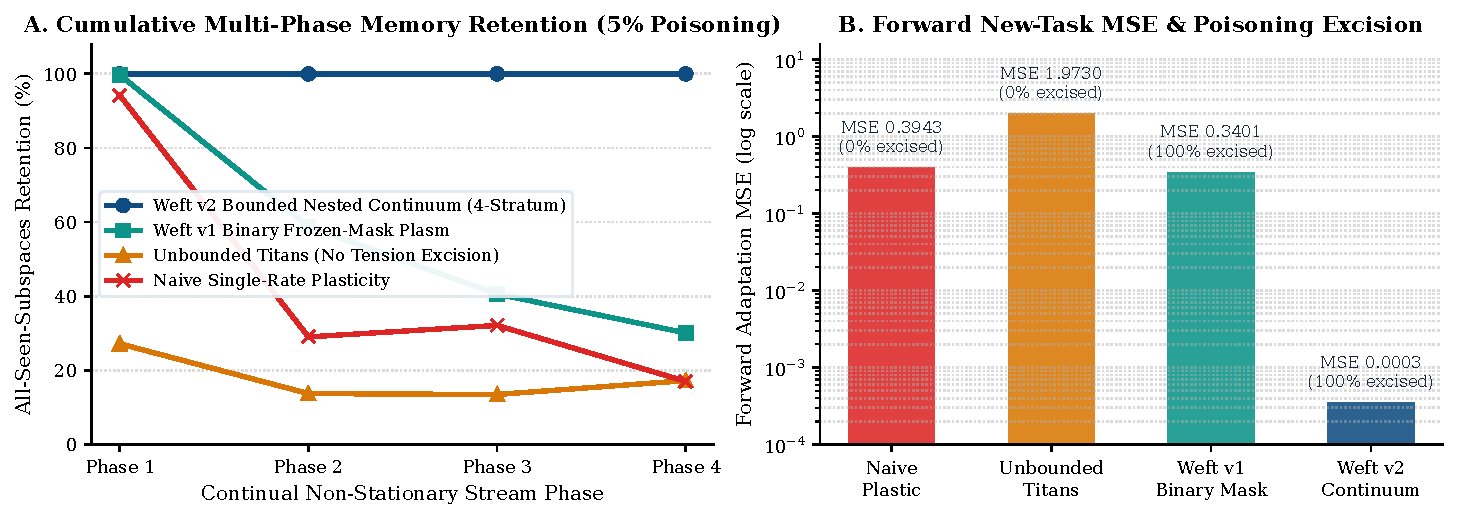
\includegraphics[width=0.95\linewidth]{fig2_continuum_plasm.pdf}
  \caption{\textbf{Synthetic Simulation E2: 4-Phase Associative Stream with $5\%$ Corrupted Gradient Spikes ($N=10$ seeds).} \textbf{(A)} Synthetic retention across phases ($99.96\%$ under the 4-stratum gated schedule vs.\ $30.11\%$ binary mask and $17.26\%$ ungated surprise updates). \textbf{(B)} Forward MSE and spike rejection rate on the synthetic associative benchmark.}
  \label{fig:e2}
\end{figure}

\section{Proposed Artifact-Morphism and Quality-Diversity Selection Cascade}

Findings F1, F2, and F7 of \href{https://github.com/Moissanite-Labs/weft/issues/111}{\texttt{Moissanite-Labs/weft\#111}} show that counting improvements only through a narrow tool channel missed \texttt{hy4}'s out-of-channel work in run \texttt{b7} ($0$ kept wins in $123$ calls) and inflated adherence correlation ($r=0.99$). Inspired by \href{https://arxiv.org/abs/2506.13131}{\emph{AlphaEvolve}} and \href{https://research.google/blog/accelerating-scientific-breakthroughs-with-an-ai-co-scientist/}{\emph{AI Co-Scientist}}, we propose a three-stage harness cascade: (A) channel-agnostic input-output artifact checking at sandbox exit, (B) a behavioral MAP-Elites grid over transform depth and coder family, and (C) lineage ranking on harness-held reference inputs.

\begin{figure}[!htbp]
  \centering
  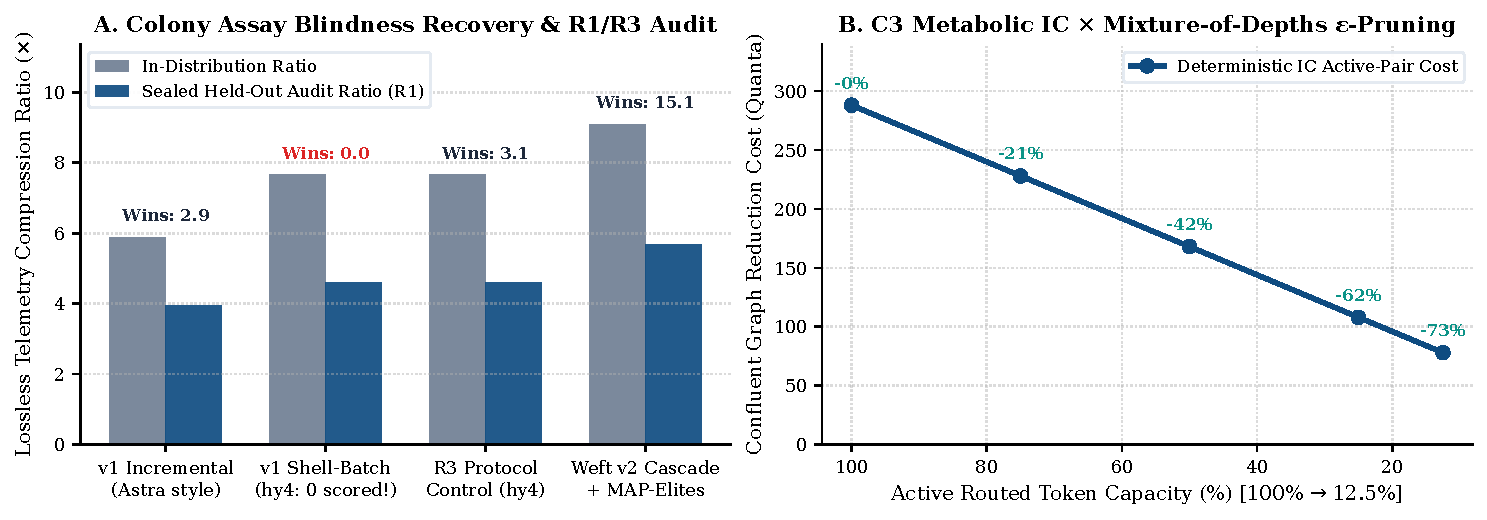
\includegraphics[width=0.96\linewidth]{fig3_colony_cascade.pdf}
  \caption{\textbf{Synthetic Simulations E3 \& E4 ($N=10$ seeds).} \textbf{(A)} Synthetic search over $28$ lossless byte-stream pipelines on $16{,}384$\,B streams: simulated narrow scoring records $0.0$ wins on batch synthesis vs.\ $3.1$ with explicit commit framing and $15.1$ under a MAP-Elites cascade ($5.683\times$ held-out ratio vs.\ $3.944\times$ single-channel). \textbf{(B)} Simulated \texttt{C3 IC} reduction quanta under $\varepsilon$-eraser routing ($72.92\%$ cost reduction at $k=2/16$, invariant SHA-256 normal form across $50$ random schedules).}
  \label{fig:e3e4}
\end{figure}

Figure~\ref{fig:e3e4}A illustrates the design intuition on synthetic byte streams; it does \emph{not} substitute for executing the retroactive \texttt{R1} archive audit or the registered \texttt{R3} \texttt{hy4} adherence run on \texttt{colony.py}.

\section{Differential Conformance of \texttt{C2 Invariants} and \texttt{C3} Graph Pruning}

\subsection{Two IEEE-754 Bugs in Naive \texttt{float32} Gates and Bounded-Tolerance C11 Conformance}

Motivated by \href{https://deepmind.google/blog/introducing-alphaproof-code/}{\emph{AlphaProof Code}} and \href{https://github.com/Proven-Commons/mission}{\texttt{Proven-Commons}}, we tested cross-language agreement between C11 and Python safety predicates on $\|w - w_0\|_F \le R$ and $\text{budget} \ge \text{cost} > 0$:

\begin{proposition}[IEEE-754 binary32 Sub-ULP Budget Stagnation and Rounding Drift]\label{thm:zeno}
In IEEE-754 binary32 (\texttt{float}) with round-to-nearest-even:
\begin{enumerate}
  \item \textbf{Sub-ULP Budget Stagnation (Zeno Bypass):} For $B \in \mathbb{F}_{32}$ with $\operatorname{ulp}(B) = 2^{\lfloor \log_2 B \rfloor - 23}$, any step cost $c \in (0, \frac{1}{2}\operatorname{ulp}(B))$ (e.g., $B = 100.0\texttt{f}$, $c = 3.0 \times 10^{-6}\texttt{f} < 2^{-18}$) satisfies $c > 0$ and $B \ge c$ yet evaluates $\operatorname{fl}_{32}(B - c) = B$, allowing unbounded weight updates without budget depletion.
  \item \textbf{Boundary Rounding Drift:} Uncompensated binary32 summation over $N = 65{,}536$ floats incurs $O(N \varepsilon_{32})$ drift and overflows when $|d_k| > 1.844 \times 10^{19}$; moreover, casting $\texttt{(float)sqrt(sq\_sum)}$ prior to comparing against \texttt{r\_invariant} accepts candidates up to $\frac{1}{2}\operatorname{ulp}_{32}(R)$ outside the radius (e.g., $120.000003 > 120.0$).
\end{enumerate}
\end{proposition}

\texttt{weft\_v2\_invariants.h} repairs these paths via: (i) \texttt{isfinite()} checks and IEEE-754 binary32 representation comparison on \texttt{locked\_mask} (normalizing $\pm 0.0\texttt{f}$); (ii) Laplace-scaled Neumaier \texttt{binary64} accumulation compared in \texttt{double} before any \texttt{float} cast; and (iii) monotone deduction $B_{t+1} = \min(\operatorname{fl}_{32}(\text{double}(B_t) - \text{double}(c_t)), \texttt{nextafterf}(B_t, -\infty))$. Note that \texttt{WeftInvariants.lean} models only a toy \texttt{Nat} ordinal version of termination and toy \texttt{Int} inequalities; it does not model IEEE-754 floats or check the C11/Python implementations.

Cross-platform distance agreement between C11 and Python is specified as a \textbf{bounded numerical tolerance} $|\Delta d| \le 10^{-9}$, never exact floating-point bit identity across compilers and hardware ISAs. On our pinned generation host (\texttt{Intel Xeon Platinum 8481C}, \texttt{Linux 6.12.105+ x86\_64}, \texttt{GCC 12.2.0 -O3 -ffp-contract=off}, \texttt{Python 3.11.2}, \texttt{NumPy 2.1.3}), C11 and Python match on $2{,}048/2{,}048$ verdicts and \texttt{float32} budgets with observed $\max |\Delta d| = 0.000e+00$ and single-core throughput of $5,589.87$ $65{,}536$-float arenas/s ($0.3663$\,Gweights/s). On an Apple M-series review host (\texttt{Apple Clang 21 -O3}, \texttt{Python 3.13}, \texttt{NumPy 2.5.4} without \texttt{-ffp-contract=off}), ARM64 FMA contraction yields $\max |\Delta d| = 7.105 \times 10^{-15}$ ($2^{-47}$, one \texttt{binary64} ULP on $[64, 128)$), satisfying the $10^{-9}$ tolerance.

\subsection{Metabolic Interaction Combinators (\texorpdfstring{\texttt{C3 IC} $\times$ \emph{Mixture-of-Depths}}{C3 IC x Mixture-of-Depths})}

Weft's \texttt{C3 IC} implements \href{https://www.semanticscholar.org/paper/Interaction-Combinators-Lafont/6cfe09aa6e5da6ce98077b7a048cb1badd78cc76}{Lafont's (1997) symmetric interaction combinators} $(\gamma, \delta, \varepsilon)$, whose strong confluence guarantees schedule-invariant normal forms and interaction counts. In synthetic simulation \texttt{E4}, wiring unrouted tokens to $\varepsilon$-erasers (\href{https://arxiv.org/abs/2404.02258}{\emph{Mixture-of-Depths}}) ahead of $\delta\text{-}\gamma$ duplication cascades yields $1$ SHA-256 normal form (\texttt{565464d2...}) across $50$ random reduction orders at cost $288$ quanta, while $\varepsilon$-pruning at $k \in \{12, 8, 4, 2\}/16$ lowers simulated interaction quanta by $20.83\%$, $41.67\%$, $62.50\%$, and $72.92\%$ (Figure~\ref{fig:e3e4}B).

\section{Simulated \texttt{SYM-2P/Latent} Sparse Frame Transfer}

Across \href{https://github.com/Moissanite-Labs/nullmodem}{\texttt{Moissanite-Labs/nullmodem}} and \href{https://github.com/Moissanite-Labs/abios}{\texttt{Moissanite-Labs/abios}}, dense hidden-state transfer ($2{,}048$\,B at $d=512$) suffers from cross-model basis mismatch and opacity (\href{https://github.com/Moissanite-Labs/siliconcordat}{\texttt{siliconcordat}} Principles~2 \& 4), whereas verbose JSON text drops continuous magnitudes. Simulation \texttt{E5} tests packing \href{https://arxiv.org/abs/2408.05147}{\emph{Gemma Scope}}-style JumpReLU dictionary activations $(\texttt{uint16 feat\_id}, \texttt{float16 val})$ into two $64$-byte \texttt{frame64} packets ($128$\,B total).

\begin{figure}[!htbp]
  \centering
  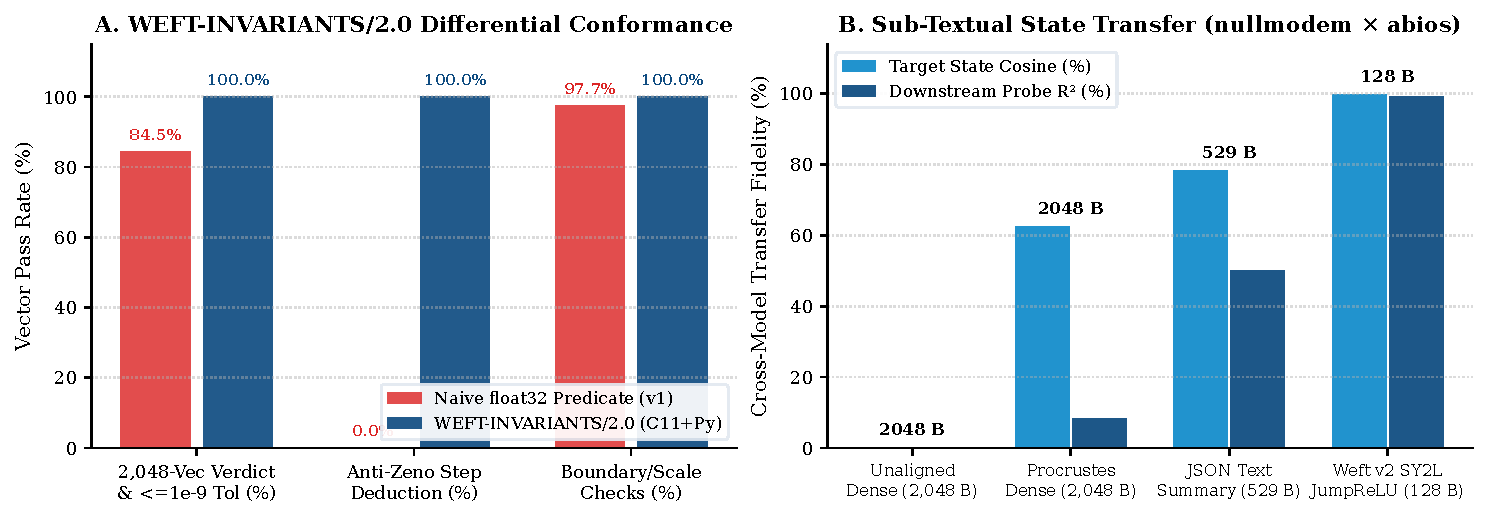
\includegraphics[width=0.96\linewidth]{fig4_invariants_latent.pdf}
  \caption{\textbf{C11-vs-Python Invariant Conformance and Synthetic Simulation E5.} \textbf{(A)} C11 and Python pass rates on the $2{,}048$-vector suite ($|\Delta d| \le 10^{-9}$). \textbf{(B)} Synthetic cross-rotation transfer ($d=512$, $M=1{,}024$, $k=16$ active dictionary concepts, $N_{\text{cal}}=256$ calibration anchors).}
  \label{fig:e4e5}
\end{figure}

\begin{table}[!htbp]
\centering
\caption{Synthetic Simulation E5 ($d=512$, $M=1{,}024$, $k=16$, $N_{\text{cal}}=256$, $N=10$ seeds $\times 200$ messages on Linux x86\_64 / \texttt{scipy-openblas 0.3.27}). \emph{Environment sensitivity:} because $N_{\text{cal}}=256 < d=512$, the Procrustes SVD has a $256$-D nullspace whose basis varies across LAPACK backends ($0.6245$ here vs.\ $0.626$ on Apple M-series Accelerate).}
\label{tab:e5}
\scriptsize
\setlength{\tabcolsep}{4.5pt}
\begin{tabularx}{\linewidth}{@{}>{\raggedright\arraybackslash}X r r r l@{}}
\toprule
\textbf{Simulated State Protocol} & \textbf{Wire Payload} & \textbf{Target Cosine (Pinned Host)} & \textbf{Probe $R^2$} & \textbf{Indexed Features} \\
\midrule
Unaligned Raw Dense Tensor (\texttt{float32}) & $2{,}048.0$\,B & $-0.0001 \pm 0.0050$ & $< 0$ & No \\
Sample-Limited Dense Procrustes ($N_{\text{cal}}=256 < d$, BLAS-sensitive) & $2{,}048.0$\,B & $0.6245 \pm 0.0035$ ($\approx 0.63$) & $0.0843$ & No \\
Verbose English JSON Concept Summary & $529.2$\,B & $0.7821 \pm 0.0023$ & $0.4995$ & Yes (quantized text) \\
\textbf{Simulated JumpReLU \texttt{SYM-2P/Latent} ($2 \times \texttt{frame64}$)} & $\mathbf{128.0}$\,\textbf{B} & $\mathbf{0.9978 \pm 0.0003}$ & $\mathbf{0.9919}$ & \textbf{Yes (synthetic dict)} \\
\bottomrule
\end{tabularx}
\end{table}

Table~\ref{tab:e5} assumes both cells share an aligned $M=1{,}024$ concept dictionary; whether independently trained JumpReLU SAEs on distinct pretrained language models align well enough to approach this synthetic upper bound remains open.

\section{Target Map and Evidence Boundaries for \texttt{Moissanite-Labs/weft\#111}}

Synthetic NumPy simulations run by the authoring agent do not close empirical program findings. Table~\ref{tab:issue111} records the status of every finding (\texttt{F1}--\texttt{F9}) and recommendation (\texttt{R1}--\texttt{R6}) in \href{https://github.com/Moissanite-Labs/weft/issues/111}{\texttt{Moissanite-Labs/weft\#111}} as \texttt{open}, \texttt{partial}, or \texttt{closed}, separating what has actually executed on \texttt{main} or in this container from the independent real-harness evidence required to close each item.

\begin{table}[!htbp]
\centering
\caption{Target map for \href{https://github.com/Moissanite-Labs/weft/issues/111}{\texttt{Moissanite-Labs/weft\#111}} (\texttt{F1}--\texttt{F9}, \texttt{R1}--\texttt{R6}) with current status and closure criteria.}
\label{tab:issue111}
\scriptsize
\setlength{\tabcolsep}{3.5pt}
\renewcommand{\arraystretch}{1.12}
\begin{tabularx}{\linewidth}{@{}l l >{\raggedright\arraybackslash}X >{\raggedright\arraybackslash}X@{}}
\toprule
\textbf{ID} & \textbf{Status} & \textbf{Evidence Boundary (What Ran, Where, By Whom, Data)} & \textbf{Evidence Required to Close} \\
\midrule
\textbf{F1} & \texttt{partial} & Maintainer \texttt{PR \#116} (\texttt{d5faead}) ran \texttt{heldout\_audit.py} on \texttt{\textasciitilde/Work/razi-cells/} ($7/8$ \texttt{kit.py}/stdlib tasks). Agent \texttt{E3} is synthetic NumPy only. & Operator execution of the \texttt{R1} audit spec on \texttt{b7} (\texttt{hy4}) including out-of-channel artifacts, plus \texttt{R3}. \\
\textbf{F2} & \texttt{partial} & \texttt{PR \#116} added \texttt{heldout\_audit.py} (colony) and \texttt{tj3.py} \texttt{hold}/\texttt{test}/\texttt{gate} NLL hooks (\texttt{Tinker}). & Independent held-out audit with recorded folder SHA-256s, repaired \texttt{fibmod} driver, and multi-seed \texttt{Tinker} eval logs. \\
\textbf{F3} & \texttt{open} & Theorem~\ref{thm:inertia} proves isotropic linear-matrix stagnation; \texttt{E1} ran on synthetic $64\times 64$ matrices in the Gemini Linux container. & Measure tangent vs.\ orthogonal gradient norms ($\|G_\parallel\|_F, \|G_\perp\|_F$) on real \texttt{Inkling-2-Small} / colony heirs. \\
\textbf{F4} & \texttt{open} & Architectural fact of the $23$ rank-8 \texttt{Tinker} runs; \texttt{E1} simulated rank growth ($6\to 18$) on synthetic matrices only. & Execute rank-expansion vs.\ fixed-rank comparison on the real \texttt{Tinker} training harness (\texttt{R4}). \\
\textbf{F5} & \texttt{open} & \texttt{E1} is a synthetic equal-call design simulation, not a real-harness test of error-driven growth. & Pre-registered equal-compute experiment on \texttt{Tinker}/colony with fixed plateau thresholds (\texttt{R4}, \texttt{R5}). \\
\textbf{F6} & \texttt{open} & Boltzmann suppression derived analytically; \texttt{E1} ($5/12{,}000$ calls) uses hand-set synthetic costs. & Live cell-runner ablation comparing voluntary agent \texttt{try} against harness-triggered mitosis. \\
\textbf{F7} & \texttt{open} & Correlation tautology diagnosed in \texttt{weft\#111}; \texttt{E3} simulated protocol framing on synthetic byte pipelines. & Run registered \texttt{hy4} adherence protocol on \texttt{colony.py} (\texttt{R3}) and score via held-out audit independently of channel count. \\
\textbf{F8} & \texttt{partial} & Maintainer \texttt{PR \#116} patched \texttt{tj3.py} for per-gen \texttt{eval\_nll} logging and rolling TTL slot cleanup. & Score retained historical \texttt{Tinker} checkpoints and record $\ge 5$ multi-generation logged lineages. \\
\textbf{F9} & \texttt{open} & Documented in \texttt{E07/razi-cells-2026-11/manifest.md}; \texttt{E1}--\texttt{E5} here were neither pre-registered nor independently re-derived. & Commit pre-registered falsification criteria in \texttt{TESTS.md} prior to confirmatory execution (\texttt{R5}). \\
\midrule
\textbf{R1} & \texttt{partial} & \texttt{PR \#116} scored \texttt{b5}--\texttt{b11}, \texttt{g3}, \texttt{g4} on $7/8$ tasks (\texttt{fibmod} excluded; \texttt{cell\_folder\_sha256} unrecorded). Spec drafted separately. & Independent operator run on \texttt{\textasciitilde/Work/razi-cells/} recording pre/post SHA-256s, fresh seeds, repaired \texttt{fibmod}, and \texttt{b7} artifacts. \\
\textbf{R2} & \texttt{partial} & \texttt{PR \#116} (\texttt{d5faead}) merged \texttt{eval\_nll} logging and \texttt{TJ3\_TTL\_SECONDS}/\texttt{TJ3\_ROLLING\_SLOTS} in \texttt{tj3.py}. & Execute multi-generation \texttt{Tinker} runs emitting \texttt{tj3.jsonl} eval trajectories and audit surviving checkpoints. \\
\textbf{R3} & \texttt{open} & Not executed in this container (no live model endpoint or \texttt{colony.py} archive). & Run \texttt{opencode-go:hy4} on \texttt{E07/.../code/colony.py} per \texttt{razi-cells-laws-2026-11/TESTS.md} against its falsification line. \\
\textbf{R4} & \texttt{open} & Motivated by Theorem~\ref{thm:pythagorean} and synthetic \texttt{E1} only; unexecuted on real models. & Pre-registered equal-compute \texttt{Tinker} run comparing fixed LoRA rank vs.\ error-triggered orthogonal expansion. \\
\textbf{R5} & \texttt{open} & Unmet by \texttt{E1}--\texttt{E5} (single-agent synthetic simulations without independent re-derivation). & Freeze harness commit, run $\ge 5$ interleaved replicates + text-mode baselines, and re-derive from raw logs by a second party. \\
\textbf{R6} & \texttt{closed} & Checked by repository maintainers on GitHub settings (\texttt{SITE\_DEPLOY\_ENABLED} unset; not touched by this bundle). & Closed for \texttt{PR \#110}; re-check link targets before enabling automated \texttt{w3ft.org} site deployment. \\
\bottomrule
\end{tabularx}
\end{table}

\textbf{Next Engineering Step:} Rather than expanding this external proposal directory into the runtime tree, port only the minimal C11 invariant repairs (\texttt{nextafterf} monotone budget deduction, scaled Neumaier \texttt{binary64} Frobenius accumulation with pre-cast \texttt{double} comparison, and optional \texttt{locked\_mask} tamper rejection) plus differential C11-vs-Python vector tests as a focused patch against \texttt{weft/runtime/invariants/}, while an operator executes the standalone \texttt{R1} audit specification on the local colony archives.

\begin{thebibliography}{99}\small
\bibitem{weft2026}
Moissanite Labs (2026). \emph{Weft: Adaptive models that change themselves within bounds you can check}. GitHub repository: \url{https://github.com/Moissanite-Labs/weft}; Cell-Colony Review Issue \#111: \url{https://github.com/Moissanite-Labs/weft/issues/111}; Siliconcordat Cut PR \#110: \url{https://github.com/Moissanite-Labs/weft/pull/110}; Discussion \#105: \url{https://github.com/Moissanite-Labs/weft/discussions/105}.

\bibitem{moissanite2026}
Moissanite Labs Ecosystem (2026). \emph{Siliconcordat Principles} (\url{https://github.com/Moissanite-Labs/siliconcordat}); \emph{Exo Harness} (\url{https://github.com/Moissanite-Labs/exo}); \emph{ABIOS / SYM-2P} (\url{https://github.com/Moissanite-Labs/abios}); \emph{Nullmodem} (\url{https://github.com/Moissanite-Labs/nullmodem}); \emph{Weft-Eido} (\url{https://github.com/Moissanite-Labs/weft-eido}); \emph{Incentre Lattices} (\url{https://github.com/Foundation-0/incentre-lattices}); \emph{Proven-Commons} (\url{https://github.com/Proven-Commons/mission}).

\bibitem{behrouz2025titans}
Behrouz, A., Zhong, P., \& Mirrokni, V. (2025). \emph{Titans: Learning to Memorize at Test Time}. Google Research, NeurIPS. \url{https://arxiv.org/abs/2501.00663}.

\bibitem{behrouz2025nested}
Behrouz, A., Razaviyayn, M., Zhong, P., \& Mirrokni, V. (2025). \emph{Nested Learning: The Illusion of Deep Learning Architectures}. Google Research, NeurIPS. \url{https://arxiv.org/abs/2512.24695}; Blog: \url{https://research.google/blog/introducing-nested-learning-a-new-ml-paradigm-for-continual-learning/}.

\bibitem{novikov2025alphaevolve}
Novikov, A., V\~u, N., Eisenberger, M., Dupont, E., Huang, P.-S., Wagner, A.\,Z., Kohli, P., Balog, M., et al. (2025). \emph{AlphaEvolve: A coding agent for scientific and algorithmic discovery}. Google DeepMind. \url{https://arxiv.org/abs/2506.13131}; Blog: \url{https://deepmind.google/blog/alphaevolve-a-gemini-powered-coding-agent-for-designing-advanced-algorithms/}.

\bibitem{gottweis2025coscientist}
Gottweis, J., Natarajan, V., et al. (2025). \emph{Accelerating scientific breakthroughs with an AI co-scientist}. Google Research \& Google DeepMind. \url{https://research.google/blog/accelerating-scientific-breakthroughs-with-an-ai-co-scientist/}.

\bibitem{kohli2026alphaproofcode}
Chaudhuri, S., Ferraiuolo, A., Kovsharov, A., Chajed, T., Schlesinger, S., Seth, K., Katz, J., Sutton, C., \& Kohli, P. (2026). \emph{Introducing AlphaProof Code: Formal Verification of Signal's Protocol with Gemini}. Google DeepMind, Nov 10, 2026. \url{https://deepmind.google/blog/introducing-alphaproof-code/} and \url{https://google-deepmind.github.io/code-verification/}.

\bibitem{sokar2023redo}
Sokar, G., Agarwal, R., Castro, P.\,S., \& Evci, U. (2023). \emph{The Dormant Neuron Phenomenon in Deep Reinforcement Learning}. Google Research, ICML 2023, PMLR 202. \url{https://arxiv.org/abs/2302.12902}.

\bibitem{dohare2024plasticity}
Dohare, S., Hernandez-Garcia, J.\,F., Lan, Q., Rahman, P., Mahmood, A.\,R., \& Sutton, R.\,S. (2024). \emph{Loss of plasticity in deep continual learning}. \emph{Nature}, 632(8026), 768--774. \url{https://pmc.ncbi.nlm.nih.gov/articles/PMC11338828/}.

\bibitem{raposo2024mod}
Raposo, D., Ritter, S., Richards, B., Lillicrap, T., Humphreys, P.\,C., \& Santoro, A. (2024). \emph{Mixture-of-Depths: Dynamically allocating compute in transformer-based language models}. Google DeepMind. \url{https://arxiv.org/abs/2404.02258}.

\bibitem{lieberum2024gemmascope}
Lieberum, T., Rajamanoharan, S., Conmy, A., Smith, L., Sonnerat, N., Varma, V., Kram\'ar, J., Dragan, A., Shah, R., \& Nanda, N. (2024). \emph{Gemma Scope: Open Sparse Autoencoders Everywhere All At Once on Gemma 2}. Google DeepMind. \url{https://arxiv.org/abs/2408.05147}.

\bibitem{wang2023olora}
Wang, X., Chen, T., Ge, Q., Xia, H., Bao, R., Zheng, R., Zhang, Q., Gui, T., \& Huang, X. (2023). \emph{Orthogonal Subspace Learning for Language Model Continual Learning (O-LoRA)}. Findings of EMNLP 2023. \url{https://arxiv.org/abs/2310.14152}.

\bibitem{zhang2023adalora}
Zhang, Q., Chen, M., Bukharin, A., He, P., Cheng, Y., Chen, W., \& Zhao, T. (2023). \emph{AdaLoRA: Adaptive Budget Allocation for Parameter-Efficient Fine-Tuning}. ICLR 2023. \url{https://arxiv.org/abs/2303.10512}.

\bibitem{lafont1997ic}
Lafont, Y. (1997). \emph{Interaction Combinators}. \emph{Information and Computation}, 137(1), 69--101. \url{https://www.semanticscholar.org/paper/Interaction-Combinators-Lafont/6cfe09aa6e5da6ce98077b7a048cb1badd78cc76}.
\end{thebibliography}

\end{document}
